% Copyright 2004 by Till Tantau <tantau@users.sourceforge.net>.
%
% In principle, this file can be redistributed and/or modified under
% the terms of the GNU Public License, version 2.
%
% However, this file is supposed to be a template to be modified
% for your own needs. For this reason, if you use this file as a
% template and not specifically distribute it as part of a another
% package/program, I grant the extra permission to freely copy and
% modify this file as you see fit and even to delete this copyright
% notice. 

\documentclass{beamer}

\usepackage{biblatex}
% There are many different themes available for Beamer. A comprehensive
% list with examples is given here:
% http://deic.uab.es/~iblanes/beamer_gallery/index_by_theme.html
% You can uncomment the themes below if you would like to use a different
% one:
%\usetheme{AnnArbor}
%\usetheme{Antibes}
%\usetheme{Bergen}
\usetheme{Berkeley}
%\usetheme{Berlin}
%\usetheme{Boadilla}
%\usetheme{boxes}
%\usetheme{CambridgeUS}
%\usetheme{Copenhagen}
%\usetheme{Darmstadt}
%\usetheme{default}
%\usetheme{Frankfurt}
%\usetheme{Goettingen}
%\usetheme{Hannover}
%\usetheme{Ilmenau}
%\usetheme{JuanLesPins}
%\usetheme{Luebeck}
%\usetheme{Madrid}
%\usetheme{Malmoe}
%\usetheme{Marburg}
%\usetheme{Montpellier}
%\usetheme{PaloAlto}
%\usetheme{Pittsburgh}
%\usetheme{Rochester}
%\usetheme{Singapore}
%\usetheme{Szeged}
%\usetheme{Warsaw}

\title{Orthogonality}

% A subtitle is optional and this may be deleted
%\subtitle{Optional Subtitle}

\author{Dhruv Kohli}
% - Give the names in the same order as the appear in the paper.
% - Use the \inst{?} command only if the authors have different
%   affiliation.

\institute[Indian Institute of Technology, Guwahati] % (optional, but mostly needed)
{
  Department of Mathematics\\
  Indian Institute of Technology, Guwahati
}
% - Use the \inst command only if there are several affiliations.
% - Keep it simple, no one is interested in your street address.

\date{}
% - Either use conference name or its abbreviation.
% - Not really informative to the audience, more for people (including
%   yourself) who are reading the slides online

\subject{Stochastic Processes}
% This is only inserted into the PDF information catalog. Can be left
% out. 

% If you have a file called "university-logo-filename.xxx", where xxx
% is a graphic format that can be processed by latex or pdflatex,
% resp., then you can add a logo as follows:

% \pgfdeclareimage[height=0.5cm]{university-logo}{university-logo-filename}
% \logo{\pgfuseimage{university-logo}}

% Delete this, if you do not want the table of contents to pop up at
% the beginning of each subsection:
\AtBeginSubsection[]
{
  \begin{frame}<beamer>{Outline}
    \tableofcontents[currentsection,currentsubsection]
  \end{frame}
}

\addbibresource{ref.bib}
\setbeamertemplate{bibliography item}{}

% Let's get started
\begin{document}
\setlength{\abovedisplayskip}{1pt}
\setlength{\belowdisplayskip}{1pt}

\begin{frame}
  \titlepage
\end{frame}

\begin{frame}{Outline}
  \tableofcontents
  % You might wish to add the option [pausesections]
\end{frame}

% Section and subsections will appear in the presentation overview
% and table of contents.
\section{Motivation}
\begin{frame}{Motivation}{}
  \begin{itemize}
  \item {
    We need a basis to convert geometric calculations into algebraic calculations. An othogonal basis would make those calculations simple.
  }
  \item {
    What is the geometry of the four fundamental subspaces? It turns out that $C(A)\perp N(A^T)$ and $C(A^T)\perp N(A)$.
  }
  \item {
    If $Ax=b$ has no solution, what $x$ should be chosen? The one which minimizes the squared error $\left\|Ax-b\right\|_2$. What is the geometric and algebraic interpretation of this least squares problem. 
  }
  \item {
    How to convert any basis into orthogonal basis?
  }
  \item {
    What is the the workhorse of digital signal processing?
  }
  \end{itemize}
\end{frame}

\section{Orthogonal Vectors and Subspaces contd.}

\begin{frame}{Orthogonal Vectors and Subspaces}{}
\begin{itemize}
    \item Length $\left\|x\right\|$ in $\mathbb{R}^n$ is the positive square root of $x^Tx$. Proof by applying Pythagoras $n-1$ times.
    \item Orthogonal vectors $x^Ty = 0$. Proof by applying Pythagoras on length of sides of a right angled triangle.
    \item The inner/scalar/dot product $x^Ty = 0 \iff x \perp y$. If $x^Ty > 0$ then the angle between them is $<90$ and if $x^Ty < 0$ then angle between them is $>90$.
\end{itemize}
\begin{block}{Result $1$}
If $v_1, v_2, \ldots, v_k$ are mutually orthogonal then those vectors are linearly independent.\\
\textit{Proof - Hints}: Take dot product of $\sum_{i=1}^{k}c_iv_i = 0$  with $v_j$ and conclude that $c_j = 0$.
\end{block}
\end{frame}

\begin{frame}{Orthogonal Vectors and Subspaces contd.}
\begin{exampleblock}{Orthogonal Subspaces}
Subspaces $V$ and $W$ are orthogonal if 
\begin{equation*}
v^Tw = 0, \forall v \in V, \forall w \in W
\end{equation*}
\centering{OR}
\begin{equation*}
v^Tw = 0, \forall v \in \text{Basis}(V), \forall w \in \text{Basis}(W)
\end{equation*}
\end{exampleblock}
\begin{itemize}
    \item The subspace $\{0\}$ is orthogonal to all subspaces. A line can be orthogonal to a line or a plane but a plane cannot be orthogonal to a plane (are front and side walls of a room orthogonal?).
\end{itemize}
\end{frame}

\begin{frame}{Orthogonal Vectors and Subspaces contd.}
\begin{block}{Result $2$ - Fundamental Theorem of Orthogonality}
For a matrix $A$, $C(A) \perp N(A^T)$ and $C(A^T) \perp N(A)$.\\
\textit{Proof - Hints}: Let $x \in N(A)$ then,
\begin{align*}
    Ax = 0 \Rightarrow (\ldots \ \text{row}_j\ \ldots)^Tx = 0 \Rightarrow \text{row}_j \perp x \Rightarrow C(A^T) \perp N(A)
\end{align*}
\centering{OR}\\
Let $y = A^Tx$ (L.C. of columns of $A^T$) and $z \in N(A)$ then,
\begin{align*}
    y^Tz = x^TAz = x^T0 = 0 \Rightarrow C(A^T) \perp N(A)
\end{align*}
\end{block}
\begin{exampleblock}{Orthogonal Complement of a Subspace}
Given a subspace $V$ of $\mathbb{R}^n$. The space of all vectors orthogonal to $V$ is called orthogonal complement of $V$, denoted by $V^{\perp}$. Also,
\begin{equation*}
    \text{dim}V + \text{dim}V^{\perp} = n
\end{equation*}
\end{exampleblock}
\end{frame}

\begin{frame}{Orthogonal Vectors and Subspaces contd.}
\begin{block}{Result $3$ - Fundamental Theorem of Linear Algebra, Part 2}
Given $A_{m\times n}$, $C(A)^{\perp} = N(A^T)$ and $C(A^T)^{\perp} = N(A)$. As a result, $\text{dim}C(A)+\text{dim}N(A^T) = n, \text{dim}C(A^T) + \text{dim}N(A) = m$.\\
\textit{Proof - Hints}: We must show the following,
\begin{equation*}
    b \in C(A) \iff y^Tb = 0 \text{ whenever } y^TA = 0
\end{equation*}
$(\Rightarrow)$ Let $b = Ax$, then $y^Tb = y^TAx = 0x = 0$.\\
$(\Leftarrow)$?
\end{block}
\end{frame}

\begin{frame}{Orthogonal Vectors and Subspaces contd.}
\begin{figure}
    \centering
    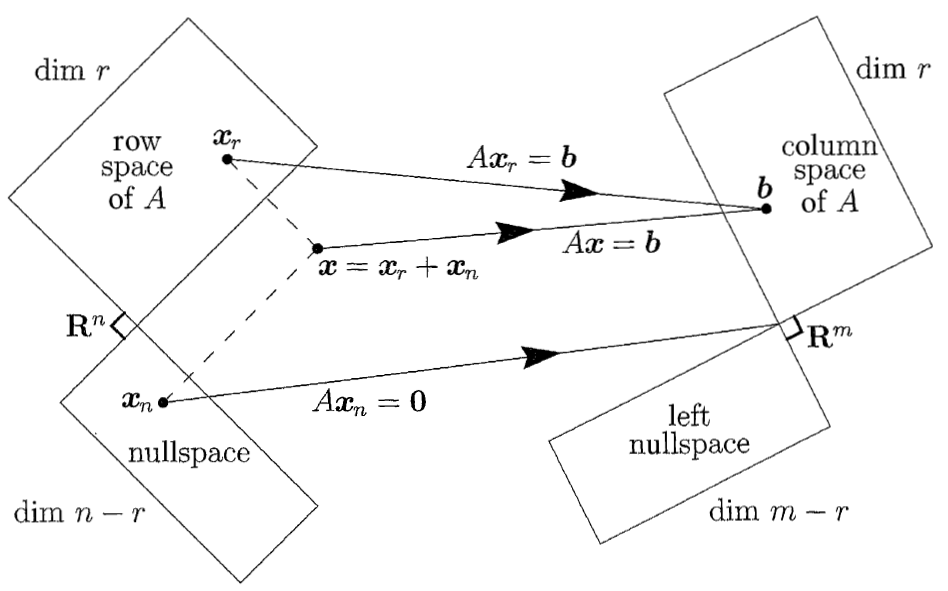
\includegraphics[scale=0.4]{fig_2}
    \caption{The true action $Ax = A(x_{\text{row}} + x_{\text{null}})$ of any $m$ by $n$ matrix.}
    \label{fig:my_label}
\end{figure}
\end{frame}

\begin{frame}{Orthogonal Vectors and Subspaces contd.}
\begin{block}{Result $4$}
From the row space to the column space, $A$ is actually invertible. Every vector $b$ in the column space comes from exactly one vector $x_r$ in the row space.\\
\textit{Proof - Hints}:
\begin{align*}
    &Ax_{r_1} = b, Ax_{r_2} = b \Rightarrow A(x_{r_1} - x_{r_2}) = 0\\
    &\Rightarrow (x_{r_1} - x_{r_2}) \in N(A) \text{ and } (x_{r_1} - x_{r_2}) \in C(A^T)\\
    &\Rightarrow x_{r_1} - x_{r_2} = 0
\end{align*}
\begin{itemize}
    \item[o] Every matrix transforms its row space onto its column space.
\end{itemize}
\end{block}
\end{frame}

% \begin{frame}{In-Lecture Exercise}

% \end{frame}

\section{Cosines and Projections onto Lines}

\begin{frame}{Cosines and Projections onto Lines}
\begin{block}{Result $5$}
The cosine of angle between any nonzero vectors $a$ and $b$ is,
\begin{equation*}
    \cos\theta = \frac{a^Tb}{\left\|a\right\|\left\|b\right\|}
\end{equation*}
\textit{Proof - Hints}: Proof by Law of Cosines
\begin{align*}
    \left\|b-a\right\| = \left\|b\right\| + \left\|a\right\| - 2\left\|b\right\|\left\|a\right\|\cos\theta
\end{align*}
\end{block}
\begin{block}{Result $6$}
The projection of vector $b$ onto the line in the direction of $a$ is,
\begin{equation*}
    p = \hat{x}a = \frac{a^Tb}{a^Ta}a
\end{equation*}
\textit{Proof - Hints}: $(b-\hat{x}a) \perp a$
\end{block}
\end{frame}

\begin{frame}{Cosines and Projections onto Lines contd.}
\begin{block}{Result $7$ - Schwarz inequality: $|a^Tb| \leq \left\|a\right\|\left\|b\right\|$}
\textit{Proof - Hints}: $\left\|e\right\| = \left\|b-p\right\| \geq 0$ or $|\cos\theta| \leq 1$
\begin{itemize}
    \item[o] Equality holds iff $b$ is a multiple of $a$ i.e. $\theta = 0 \text{ or } 180$.
\end{itemize}
\end{block}
\begin{exampleblock}{Projection Matrix}
From result $6$, matrix that projects $b$ to $a$ is given by,
\begin{align*}
    P = \frac{aa^T}{a^Ta}
\end{align*}
\begin{itemize}
    \item $P = P^T$ and $P^2 = P$ ($Pb$ already lies on the line along $a$).
    \item $C(P)$ is line through $a$ and $N(P)$ is the plane perpendicular to $a$. Note: $N(P) \perp C(P)$ because $C(P) = C(P^T)$.
    \item Rank$(P) = 1$ (Why?).
\end{itemize}
\end{exampleblock}
\end{frame}

% \begin{frame}{In-Lecture Exercise}

% \end{frame}

\section{Projection and Least Squares}

\begin{frame}{Projection and Least Squares}
\begin{itemize}
    \item For system $A_{m\times n}x = b$, if number $m$ of observations (rows) is larger than the number $n$ of unknowns, it must be expected that $Ax=b$ will be inconsistent.
    \item Probably, there will not exist a choice of $x$ that perfectly fits  data $b$. In other words, $b$ probably will not be in $C(A)$.
    \item The problem reduces to finding $\hat{x}$ that minimizes error $E = \left\|Ax-b\right\|$. This is exactly the distance between $b$ and the point $Ax$ in the column space.
    \item Need to locate $p = A\hat{x}$ that is closer to $b$ than any other point in C(A). The error vector $e = b - A\hat{x}$ must be perpendicular to $C(A)$ i.e. must lie in $N(A^T)$.
\end{itemize}
\begin{align*}
    A^T(A\hat{x}-b) = 0 \Rightarrow A^TA\hat{x} = A^Tb
\end{align*}
\end{frame}

\begin{frame}{Projection and Least Squares contd.}
\begin{itemize}
    \item Calculus way to prove is by taking derivative of $(Ax-b)^T(Ax-b)$ wrt $x$ and equating to $0$.
\end{itemize}
\begin{exampleblock}{Least Squares Problems with Several Variables}
When $Ax=b$ is inconsistent, its least-squares solution minimizes $\left\|Ax-b\right\|^2$:
\begin{align*}
    A^TA\hat{x} = A^Tb
\end{align*}
$A^TA$ is invertible $\iff$ the columns of $A$ are linearly independent\footnote{rank$(A)$+rank$(B)-n \leq $ rank$(AB) \leq \min($rank$(A),$rank$(B))$}. Then,
\begin{align*}
    \hat{x} = (A^TA)^{-1}A^Tb
\end{align*}
The projection of $b$ onto the $C(A)$ is the nearest point $A\hat{x}$:
\begin{align*}
    p = A\hat{x} = A(A^TA)^{-1}A^Tb
\end{align*}
\end{exampleblock}
\end{frame}

\begin{frame}{Projection and Least Squares contd.}
\begin{itemize}
    \item If $b \in C(A)$, ($b=Ay$), then $p = A(A^TA)^{-1}A^Tb = Ay$.
    \item If $b \in N(A^T)$, then, $p = 0$.
    \item If $A$ is invertible, then, $p = b$.
\end{itemize}
\begin{block}{Result $8$}
The cross product matrix $A^TA$ has same null space as $A$.\\
\textit{Proof - Hints}:
\begin{align*}
    A^TAx = 0 \Rightarrow x^TA^TAx = x^T0 = 0 \Rightarrow \left\|Ax\right\| = 0 \Rightarrow Ax = 0
\end{align*}
\end{block}
\begin{block}{Result $9$}
If $A_{m\times n}$ has independent columns then $A^TA$ is square, symmetric,  invertible and positive definite.\\
\textit{Proof - Hints}: Rank$(A^TA) = n$.
\end{block}
\end{frame}

\begin{frame}{Projection and Least Squares contd.}
\begin{block}{Result $10$}
Matrix $P = A(A^TA)^{-1}A^T$ projects onto $C(A)$ and $I-P$ projects onto $N(A^T)$. Two properties:
\begin{enumerate}
    \item $P = P^T$
    \item $P^2 = P$
\end{enumerate}
Also, any matrix with above properties is a projection matrix.\\
\textit{Proof - Hints}: For converse, show that $Pb$ is the projection of $b$ in $C(P)$ or $(I-P)b$ is the projection of $b$ onto a space orthogonal to $C(P)$. For a general vector $Pc$ in $C(P)$, the dot product of it with $(I-P)b$ is,
\begin{align*}
    (Pc)^T(I-P)b = c^T(P^T - P^TP)b = c^T(P - P^2)b = 0
\end{align*}
Therefore, $(I-P)b$ is in a space orthogonal to $C(P)$, and $Pb$ is the projection of $b$ in $C(P)$.
\end{block}
\end{frame}

\begin{frame}{Projection and Least Squares contd.}{Weighted Least Squares}
\begin{itemize}
    \item Idea: some observations are more reliable than others. The new error looks like $E^2 = \sum_{i=1}^{m}w_i^2(a_{r_i}^Tx_i-b_i)^2$.
    \item The solution $\hat{x_w}$ minimizes this error and is a solution of the system $WAx = Wb$.
\end{itemize}
\begin{exampleblock}{Weighted Normal Equation}
The least square solution to $WAX = Wb$ is $\hat{x_w}$:
\begin{align*}
    A^TW^TWA\hat{x_w} = A^TW^TWb
\end{align*}
\end{exampleblock}
\begin{itemize}
    \item The point $A\hat{x_w}$ still point in $C(A)$ that is closest to $b$. But the term ``closest" has new meaning - all inner products $a^Tb$ are replaced by $(Wa)^T(Wb) = a^TW^TWb$. In this new sense, $A\hat{x_w} \perp b - A\hat{x_w}$.
\end{itemize}
\end{frame}

\begin{frame}{Projection and Least Squares contd.}{Weighted Least Squares}
\begin{itemize}
\item Note: if $W$ is orthogonal then $W^TW = I$.
\item The important question is the choice of $C = W^TW$. The best answer comes from the statisticians:
\begin{enumerate}
    \item If the errors in $b_i$ are independent of each other then the right weights are $w_i = \frac{1}{\sigma_i}$ where $\sigma_i$ is the variance of the error in $b_i$. Higher the variance, lesser is the reliability and hence lesser is the weight.
    \item If the errors in $b_i$ are coupled then the best unbiased matrix $C$ is the inverse of the covariance matrix - whose $i,j$ entry is the expected value of (error in $b_i$) times (error in $b_j$).
\end{enumerate}
\end{itemize}
\end{frame}

% \begin{frame}{In-Lecture Exercise}

% \end{frame}
\section{Orthogonal Basis and Gram-Schmidt}

\begin{frame}{Orthogonal Basis and Gram-Schmidt}
\begin{exampleblock}{Orthonormal Vectors}
The vectors $q_1, q_2, \ldots, q_n$ are orthonormal if
\begin{align*}
    q_i^Tq_j = \left\{\begin{matrix}1, & i = j\\0, & i \neq j\end{matrix}\right.
\end{align*}
\end{exampleblock}
\begin{exampleblock}{Orthogonal Matrices}
If $Q$ has orthonormal columns, then $Q^TQ = I$. If $Q$ is square, then it is called orthogonal matrix and $Q^T = Q^{-1}$.
\begin{itemize}
    \item[o] $Q^TQ = I$ even if $Q$ is a rectangular matrix but then $Q^T$ is only a left-inverse.
    \item Examples of orthogonal matrices - rotation matrix, permultation matrix, reflection matrix. \textbf{Every orthogonal matrix is a product of a rotation and a reflection}.
\end{itemize}
\end{exampleblock}
\end{frame}

\begin{frame}{Orthogonal Basis and Gram-Schmidt contd.}
\begin{itemize}
    \item For square $Q$, $Q^T = Q^{-1} \Rightarrow QQ^T = I$ which means that \textbf{the rows of a square matrix are orthonormal whenever the columns are} even though the rows and columns point in a completely different direction.
    \item For square $Q$ of size $n$, the columns span $\mathbb{R}^n$ so as rows.
\end{itemize}
\begin{block}{Result $11$}
Multiplication by any $Q$ (square or rectanlge) preserves length and inner produt.\\
\textit{Proof - Hints}: $x^TQ^TQy = x^Ty$.
\begin{itemize}
    \item[o] All inner products and lengths are preserved when the space is rotated or reflected.
\end{itemize}
\end{block}
\end{frame}

\begin{frame}{Orthogonal Basis and Gram-Schmidt contd.}
\begin{block}{Result $12$}
If vectors $q_1,q_2,\ldots,q_n \in \mathbb{R}^n$ form an orthonormal basis of $\mathbb{R}^n$ (or $Q$ is orthogonal) then every $b \in \mathbb{R}^n$ can be written as:
\begin{align*}
    b = \sum_{i=1}^{k}(q_i^Tb)q_i \text{ or } b = Q(Q^Tb)
\end{align*}
\textit{Proof - Hints}: 
\begin{align*}
    b = \sum_{i=1}^{n}x_iq_i \Rightarrow q_j^Tb = q_j^T(\sum_{i=1}^{n}x_iq_i) \Rightarrow x_j = q_j^Tb
\end{align*}
\centering{OR}
\begin{align*}
    Qx = b \Rightarrow x = Q^Tb \Rightarrow b = QQ^Tb
\end{align*}
\begin{itemize}
    \item[o] Every $b$ is a sum of its one-dimesnional projections onto the lines through $q$'s $\left(\frac{q_i^Tb}{q_i^Tq_i}q_i = (q_i^Tb)q_i\right)$.
\end{itemize}
\end{block}
\end{frame}

\begin{frame}{Orthogonal Basis and Gram-Schmidt contd.}
\begin{exampleblock}{Least Squares with Orthogonal Columns}
If $Q_{m\times n}$ has orthonormal columns, the least-squares solution is:
\begin{align*}
    Qx &= b, \text{ rectangular system with no solutions for most $b$}\\
    Q^TQ\hat{x} &= Q^Tb, \text{ normal equation for best $\hat{x}$ - $Q^Q = I$}\\
    \hat{x} &= Q^Tb, \text{ $\hat{x_i} = q_i^Tb$}\\
    p &= Q\hat{x}, \text{ projection of $b$ is $(q_1^Tb)q_1+\ldots+(q_n^Tb)q_n$}\\
    p &= QQ^Tb, \text{ the projection matrix is $QQ^T$}
\end{align*}
\end{exampleblock}
\begin{itemize}
    \item $m=n \Rightarrow p=b$ and $m>n \Rightarrow p$ may or may not equal $b$.
    \item For $Ax=b$, $P = A(A^TA^{-1})A^T \xrightarrow{A=Q} P = QIQ^T=QQ^T$.
    \item $P$ projects $q \in C(Q)$ to $q$ and $q' \in N(Q^T)$ to $0$ (Why)?
\end{itemize}
\end{frame}

\begin{frame}{Orthogonal Basis and Gram-Schmidt contd.}
\begin{exampleblock}{Gram-Schmidt Orthogonalization}
Input: independent vectors $a_1, a_2, \ldots, a_n$.\\
Output: orthonormal vectors $q_1, q_2, \ldots, q_n$.\\
At step $j$, it subtracts from $a_j$ its components in the directions of $q_1, q_2, \ldots, q_{j-1}$ that are already settled:
\begin{align*}
    &A_j = a_j - (q_1^Ta_j)q_1 - (q_2^Ta_j)q_2 - \ldots - (q_{j-1}^Ta_j)q_{j-1}\\
    &q_j = \frac{A_j}{\left\|A_j\right\|}
\end{align*}
\begin{itemize}
    \item[o] $A_j$'s may be normalized at the end without affecting the resulting $q$'s (Why?).
\end{itemize}
\end{exampleblock}
\end{frame}

\begin{frame}{Orthogonal Basis and Gram-Schmidt contd.}
\begin{exampleblock}{QR Factorization}
Based on Gram-Schmidt Orthogonalization, every $m\times n$ matrix with independent columns can be factored - $A = Q_{m\times n}R_{n \times n}$. The columns of $Q$ are orthonormal and $R$ is upper triangular and invertible given by:
\begin{align*}
    R_{j} = \begin{bmatrix}q_1^Ta_j&q_2^Ta_j&.&q_j^Ta_j&0&.&0\end{bmatrix}^T \Rightarrow R_{ij} = q_i^Ta_j
\end{align*}
Note: $a_j$ has no component in the direction of $q_{j+1},\ldots,q_{n}$.
\end{exampleblock}
\begin{exampleblock}{Least Squares using QR Factorization}
If the columns of $A$ are independent then $A=QR$ and
\begin{align*}
    &A^TA = R^TQ^TQR = R^TR, \ A^Tb = R^TQ^Tb\\
    &A^TA\hat{x} = A^Tb \Rightarrow R^TR\hat{x} = R^TQ^Tb \Rightarrow R\hat{x} = Q^Tb
\end{align*}
Note: Computational cost is $mn^2$ operations of Gram Schmidt.
\end{exampleblock}
\end{frame}

\begin{frame}{Orthogonal Basis and Gram-Schmidt contd.}{Function Spaces and Fourier Series}
\begin{exampleblock}{Hilbert Space and Function Space}
\begin{itemize}
    \item All vectors in $\mathbb{R}^{\infty}$ which have finite length form a vector space called \textbf{Hilbert space}.
    \item A function defined on an interval can be imagined as a vector with a whole continuum of components. All those functions that have a finite length form \textbf{function space}.
    \item The inner product of $f$ and $g$ defined on $[a,b]$ and $[c,d]$ respectively, is defined in an analogous way as:
        \begin{align*}
            (f,g) = \int_{[a,b]\cap [c,d]}f(x)g(x)dx \text{ and } (f,f) = \int_{[a,b]}f(x)^2dx
        \end{align*}
    \item[o] Orthogonality condition - $v^Tw=0, (f,g) = 0$. Schwarz inequality - $|(f,g)| \leq \left\|f\right\|\left\|g\right\|, \ (f,f) = \left\|f\right\|^2$ (Why?).
\end{itemize}
\end{exampleblock}
\end{frame}

\begin{frame}{Orthogonal Basis and Gram-Schmidt contd.}{Function Spaces and Fourier Series}
\begin{itemize}
    \item Note: $\sin x$ and $\cos x, x \in [0,2\pi]$ are orthogonal.
\end{itemize}
\begin{exampleblock}{Fourier Series}
\textit{$(*)$ sines and cosines defined on $[0,2\pi]$ are mutually orthogonal}.
Fourier series of $f(x)$ is its expansion into sines and cosines:
\begin{align*}&
    f(x) = a_0 + a_1\cos x + b_1\sin x + a_2 \cos 2x + b_2\sin 2x + \ldots\\
    & a_0 = \frac{(f,1)}{(1,1)}, a_k = \frac{(f,\cos kx)}{(\cos kx,\cos kx)}, b_k = \frac{(f,\sin kx)}{(\sin kx,\sin kx)}, k \neq 0
\end{align*}
\begin{itemize}
    \item Inner products are computed over $[0,2\pi]$.
    \item Those coefficients are obtained by using $(*)$.
    \item Fourier series is projecting $f(x)$ onto orthogonal sines and cosines. \textit{It gives the coordinates of the "vector" $f(x)$ with respect to a set of (infinitely many) perpendicular axes.}
\end{itemize}
\end{exampleblock}
\end{frame}

\begin{frame}{Orthogonal Basis and Gram-Schmidt contd.}{Function Spaces and Fourier Series}
\begin{itemize}
    \item Suppose an approximation of a function $f(x)$ is required as a linear combination of $g_1(x),\ldots,g_{k}(x)$. For example, $f(x)$ is to be approximated with the closest polynomial of degree $2$ i.e. linear combination of $\{1,x,x^2\}$ on $[0,1]$.
    \item Since $1$ and $x^2$ are never orthogonal, $f(x)$ cannot be written as a sum of its projections on $1,x$ and $x^2$.
    \item It is virtually hopeless to solve following for $10$ degrees:
    \begin{align*}
        &Ay = b \text{ where } A= [1,x,x^2], y = [y_1,y_2,y_3]^T, b = [f(x)]\\
        &A^TA = \begin{bmatrix}(1,1)&(1,x)&(1,x^2)\\(x,1)&(x,x)&(x,x^2)\\(x^2,1)&(x^2,x)&(x^2,x^2)\end{bmatrix} = \begin{bmatrix}1&1/2&1/1\\1/2&13&1/4\\1/3&1/4&1/5\end{bmatrix}
    \end{align*}
    \item $A^TA$ (called Hilbert Matrix) is ill-conditioned - Gaussian Elimination amplifies roundoff error by $10^{13}$. The right idea is to switch to orthogonal axis by Gram-Schmidt.
\end{itemize}
\end{frame}

\begin{frame}{Orthogonal Basis and Gram-Schmidt contd.}{Function Spaces and Fourier Series}
\begin{exampleblock}{Gram-Schmidt for Functions}
The process is same as the Gram-Schmidt for vectors except that the inner products will be those of functions.
\begin{itemize}
    \item Example: Consider the functions $1, x, x^2$ defined on $[-1,1]$ (it is easier to work with symmetric intervals).
    \item G-S process can start by accepting $v_1=1$ and $v_2=x$ as first two perpendicular axes (because odd powers are perpendicular to even powers on symmetric interval.)
    \item $v_3 = x^2 - \frac{(1,x^2)}{(1,1)} - \frac{(x,x^2)}{(x,x)} = x^2 - \frac{1}{3}$ will then be third axis perpendicular to $v_1$ and $v_2$.
    \item The polynomials constructed in this way are called \textbf{Legendre Polynomials} and they are orthogonal to each other on the interval $[-1,1]$.
\end{itemize}
\end{exampleblock}
\end{frame}

% \begin{frame}{In-Lecture Exercise}

% \end{frame}

% \section{The Fast Fourier Transform}

% \begin{frame}{The Fast Fourier Transform}

% \end{frame}

% \begin{frame}{In-Lecture Exercise}

% \end{frame}

\section{Bibliography}
\begin{frame}[t]
    \frametitle{Bibliography}
    \nocite{*}
    \printbibliography
\end{frame}

\end{document}


